\newchapstyle
\chapter{Probing the current-phase relation of graphene Josephson junctions
with microwave circuits}
\label{chap:gJJ-CPR}


\begin{abstract}
	We perform extensive analysis of graphene Josephson junctions embedded in microwave circuits.
	%
	By comparing a diffusive junction at \SI{15}{\milli\kelvin} with a ballistic one at \SI{15}{\milli\kelvin} and \SI{1}{\kelvin}, we are able to reconstruct the current-phase relation.
\end{abstract}

%% Start the actual chapter on a new page.
\newpage

\section{Introduction}

\section{Circuit characterization}

Our circuit consists of a DC-bias microwave cavity formed by a coplanar waveguide (CPW) which is shunted by a large capacitor at the input, and shorted to ground on the far end by a gate-voltage ($V_g$) tunable graphene Josephson junction (gJJ), cf. Fig.\ref{fig:figure1}(a) and Refs.~\cite{schmidtBallisticGrapheneSuperconducting2018,schmidtCurrentDetectionUsing2020,bosmanBroadbandArchitectureGalvanically2015c}.
%
The circuit is connected via a bias-T, allowing both DC and RF characterization in the same cooldown.
%
The gate voltage lead is fed through a shunt capacitor of the same geometry as the capacitor at the input in order to suppress RF radiation leaking  in through or out of the gate line.

We measured two separate devices with nominally identical microwave circuits and junction designs:
%
One of the devices exhibited signatures ballistic DC-transport, which we will refer to as the \textit{ballistic device}, which is the device presented in the main text of Ref.~\cite{schmidtBallisticGrapheneSuperconducting2018}.
%
The other one, in lack of such features, will be called \textit{diffusive device}, and corresponds to the reference sample of Ref.~\cite{schmidtBallisticGrapheneSuperconducting2018}.

We extract the DC circuit parameters by applying a bias current to the JJ, using the CPW as a long capacitive lead.
%
All DC lines were equipped with $\pi$-filters in the room temperature battery powered electronics, as well as copper powder and two-stage RC filters thermally anchored to the millikelvin stage of the dilution refrigerator.
%
When exceeding a critical current, the JJ switches from the zero-voltage to the resistive state.
%
We record this switching current $I_s$ for varying gate voltages, as depicted in the top row of Fig.~\ref{fig:figure1} for the two devices at two different temperatures.
%
The DC switching current of the diffusive device ranges from a few \SI{100}{\nano\ampere} to \SI{5.5}{\micro\ampere}, similar to the hot ballistic device.
%
At base temperature, the maximum $I_s$ of the ballistic device reaches \SI{7.5}{\micro\ampere} for $V_g>V_{\rm CNP}$, while for p-doping the enhancement in $I_s$ is significantly smaller.

For high frequency signals, i.e. a few \si{\giga\hertz}, the gJJ behaves as a nonlinear inductor, with Josephson inductance
%
\begin{align}
L_J = \frac{\Phi_0}{2\pi}\left(\diff{I_J}{\delta}\right)^{-1},
\end{align}
%
where $I_J(\delta)$ is the current phase relation (CPR) between the phase difference across and the corresponding supercurrent $I_J$ flowing through the junction.
Depending on the impedance of the gJJ, $Z_J(V_g)=j\omega L_J(V_g)$, the fundamental mode hosted by the CPW+gJJ varies between a $\lambda/2$ wave for $Z_J\rightarrow0$ and $\lambda/4$ for $Z_J\rightarrow\infty$.
%
Since the supercurrent in our gJJs cannot be fully suppressed, the maximum $L_J\lessapprox\SI{1}{\nano\henry}$, thus $Z_J\lessapprox1\ll Z_0\approx\SI{50}{\ohm}$ with the CPW impedance $Z_0$.
%
Our devices thus remain in the $\lambda/2$-resonator regime.

Measurements show a gate-tunable resonance frequency $f_0$ between \SIrange{7}{8.2}{\giga\hertz}, comparable for both devices, cf. bottom row of Fig.~\ref{fig:figure1}.
%
Due to the inverse nature of junction current and inductance, the large changes in $I_s$ for $V_g>V_{\rm CNP}$ only lead to minor changes in $f_0$ when comparing the hot and cold ballistic device.
%
On the other hand, even small changes in the significantly smaller $I_s$ for $V_g<V_{\rm CNP}$ significantly reduce $f_0$ in this regime.

\begin{figure}
	\centering
	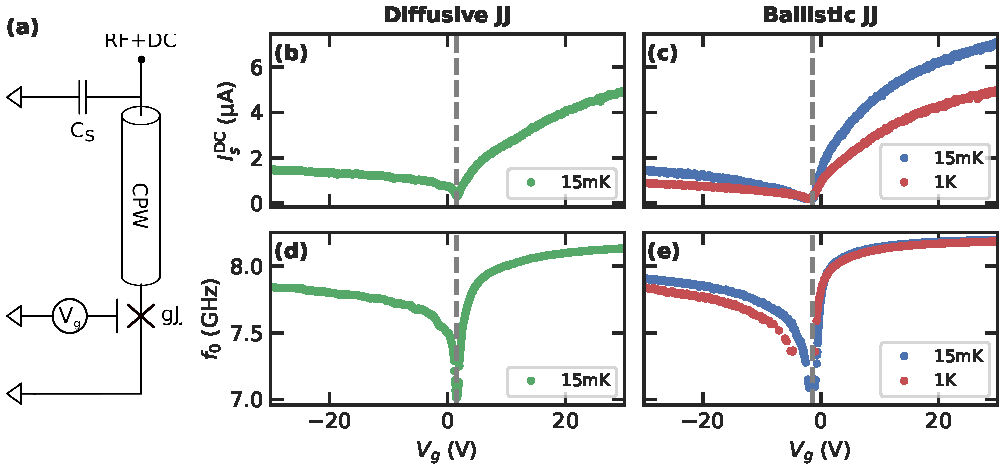
\includegraphics[width=\linewidth]{chapter-gJJ-CPR/figs/Figure1}
	\caption{
		\textbf{A graphene Josephson junction embedded in a DC bias microwave circuit.}
		%
		\textbf{(a)} Measurement schematic.
		%
		The gJJ shorts a coplanar waveguide transmission line to ground, which forms a gate-tunable $\lambda/2$-resonator.
		%
		\textbf{(b-e)} Switching currents (top row) for the diffusive \textbf{(b)} and ballistic Josephson junction \textbf{(d)}, at base-temperature of \SI{15}{\milli\kelvin} (blue) and at \SI{1}{\kelvin} (red).
		%
		Bottom row: Resonance frequencies versus gate voltage for the diffusive \textbf{(c)} and ballistic \textbf{(e)} device.
		%
		The gate-tunable Josephson inductance changes the boundary condition of the $\lambda/2$-resonator, thus changing the resonance frequency of the circuit.
		%
		Dashed grey lines indicate the charge neutrality point
	}
	\label{fig:figure1}
\end{figure}

\section{Extracting the Josephson inductance from DC and RF measurements}

The resonance frequency of a $\lambda/2$-resonator shorted to ground by a Josephson inductance can be modeled by
\begin{align}
f_0(I_b,I_c) = \frac{f_{\lambda/2}}{1 +  L_J(I_b, I_c)/L_r}
\label{eq:Pogorzalek}
\end{align}
%
with $L_r$ the bare CPW inductance and $f_{\lambda/2}$ the resonance frequency of the CPW without the JJ~\cite{pogorzalekHystereticFluxResponse2017}.
%
$I_b$ is the bias current flowing through CPW and the JJ, $I_c$ the critical current of the JJ.
%
Assuming a purely sinusoidal current-phase relation,
%
\begin{align}
I_J(\delta) = I_c\sin\delta,
\label{eq:CPR-sin}
\end{align}
%
the Josephson inductance can be extracted from the current phase relation via
%
\begin{align}
L_J = \frac{\Phi_0}{2\pi\sqrt{I_c^2-I_b^2}}.
\end{align}

As depicted in Fig.\ref{fig:figure2}, we fit the RF-measured $f_0$ versus the DC-measured $I_s$ using Eq.\ref{eq:Pogorzalek} assuming a sinusoidal CPR, shown by the black dashed line.
%
The fit converges for both the diffusive and the hot ballistic device.
%
On the other hand, at \SI{15}{\milli\kelvin}, the ballistic device exhibits multi-valued $f_0(I_s)$, as the resonance frequency and switching current follow different trends for p- and n-doping.

\begin{figure}
	\centering
	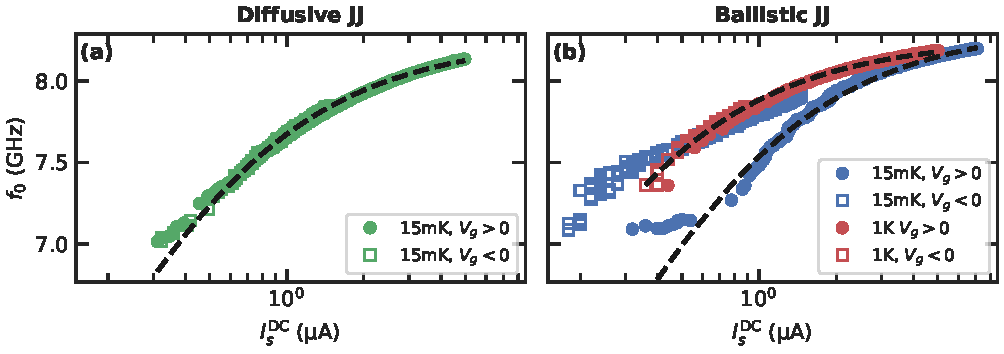
\includegraphics[width=0.5\linewidth]{chapter-gJJ-CPR/figs/Figure2}
	\caption{
		\textbf{Resonance frequency vs switching currents for two different gJJ devices.}
		%
		Both the diffusive device at low temperature \textbf{(a)} and the ballistic device at \SI{1}{\kelvin} (\textbf{(b)}, red) show monotonically increasing $f_0$ versus DC-extracted switching currents.
		%
		In contrast, for low temperatures, the ballistic gJJ (\textbf{(b)}, blue) exhibits multi-valued $f_0(I_s)$ for gate voltages larger (full circles) and smaller (empty squares) than the charge neutrality point.
		%
		The	multivalued behavior in the ballistic device at low temperature indicates a strong nonsinusoidal CPR, while this is not observed for diffusive and hot transport.
		%
		Dashed lines correspond to fits to Eq.~\ref{eq:Pogorzalek}.
	}
	\label{fig:figure2}
\end{figure}

\begin{figure}
	\centering
	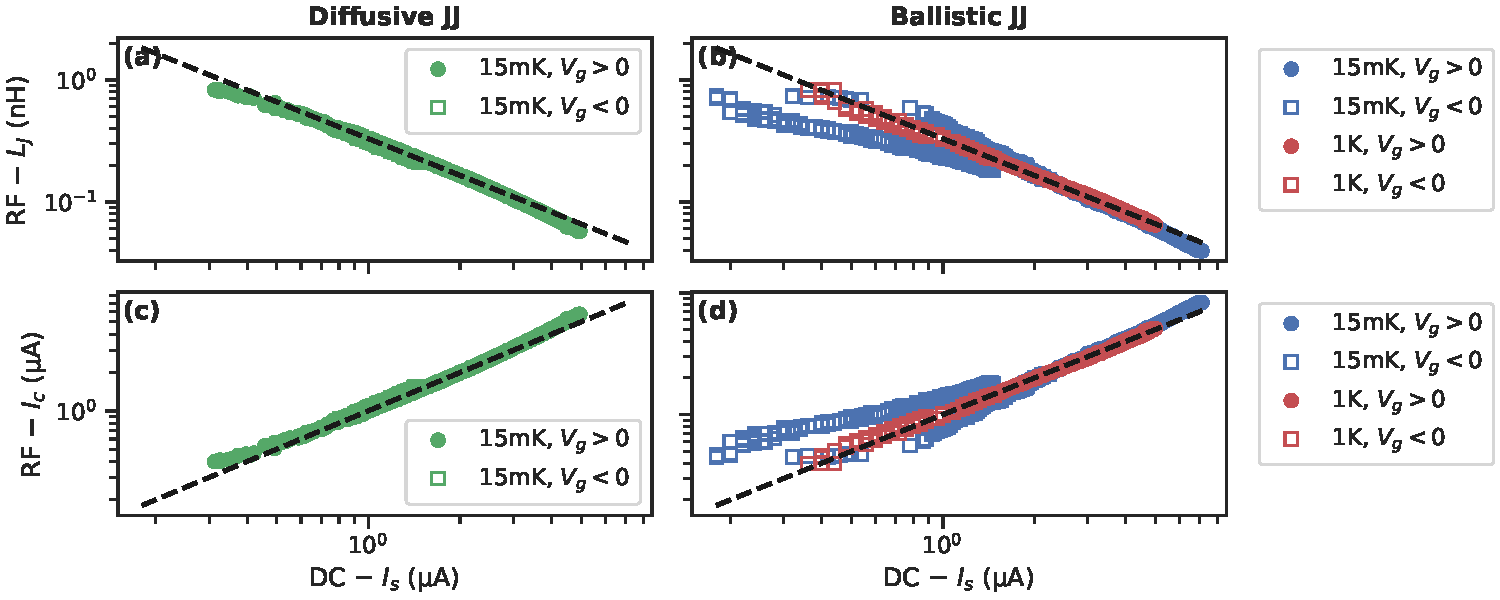
\includegraphics[width=0.833\linewidth]{chapter-gJJ-CPR/figs/Figure3}
	\caption{
		\textbf{Comparing switching current and Josephson inductance.}
		%
		Both scattering in the JJ as well as elevated temperatures reduce the deviation from RF and DC data.
		%
		\textbf{(a-b)} RF-extracted Josephson inductance versus DC-measured switching current for the diffusive device at \SI{15}{\milli\kelvin} \textbf{(a)} and ballistic device at \SI{15}{\milli\kelvin} and at \SI{1}{\kelvin} (\textbf{(b)}, blue and red, respectively).
		%
		Solid line corresponds to Josephson inductance calculated from sinusoidal CPR.
		%
		\textbf{(c-d)} Corresponding RF-extracted critical current.
		%
		Solid line corresponds to DC-measured $I_s$.
	}
	\label{fig:figure3}
\end{figure}

\section{Circuit anharmonicity}

The anharmonicity of a CPW shorted to ground by a Josephson junction is
\begin{align}
\alpha=-\frac{\omega_0}{2} \left(\frac{L_J}{L_r+L_J}\right)^3,
\end{align}
\cite{wilsonPhotonGenerationElectromagnetic2010b,zhouHighgainWeaklyNonlinear2014}
%
with $\omega_0=2\pi f_0$.
%
However, in the case of a non-sinusoidal CPR, the anharmonicity is reduced due to the increased CPR slope, resulting in
\begin{align}
\alpha^\prime = \alpha \left( 1-\frac{3}{4}\frac{\sum_i\tau_i^2}{\sum_i\tau_i}\right) \rightarrow \alpha \left( 1-\frac{3}{4}\tau \right)
\end{align}
\cite{kringhojAnharmonicitySuperconductingQubit2018}

A more suitable measurement would have been to perform two-tone spectroscopy with a fixed-frequency pump tone with variable power, and a low-power swept probe tone, since this would avoid bifurcation and yield a direct measurement of the anharmonicity from the frequency shift per photon.
%
However, such a setup was not available at the time.

\begin{figure}
	\centering
	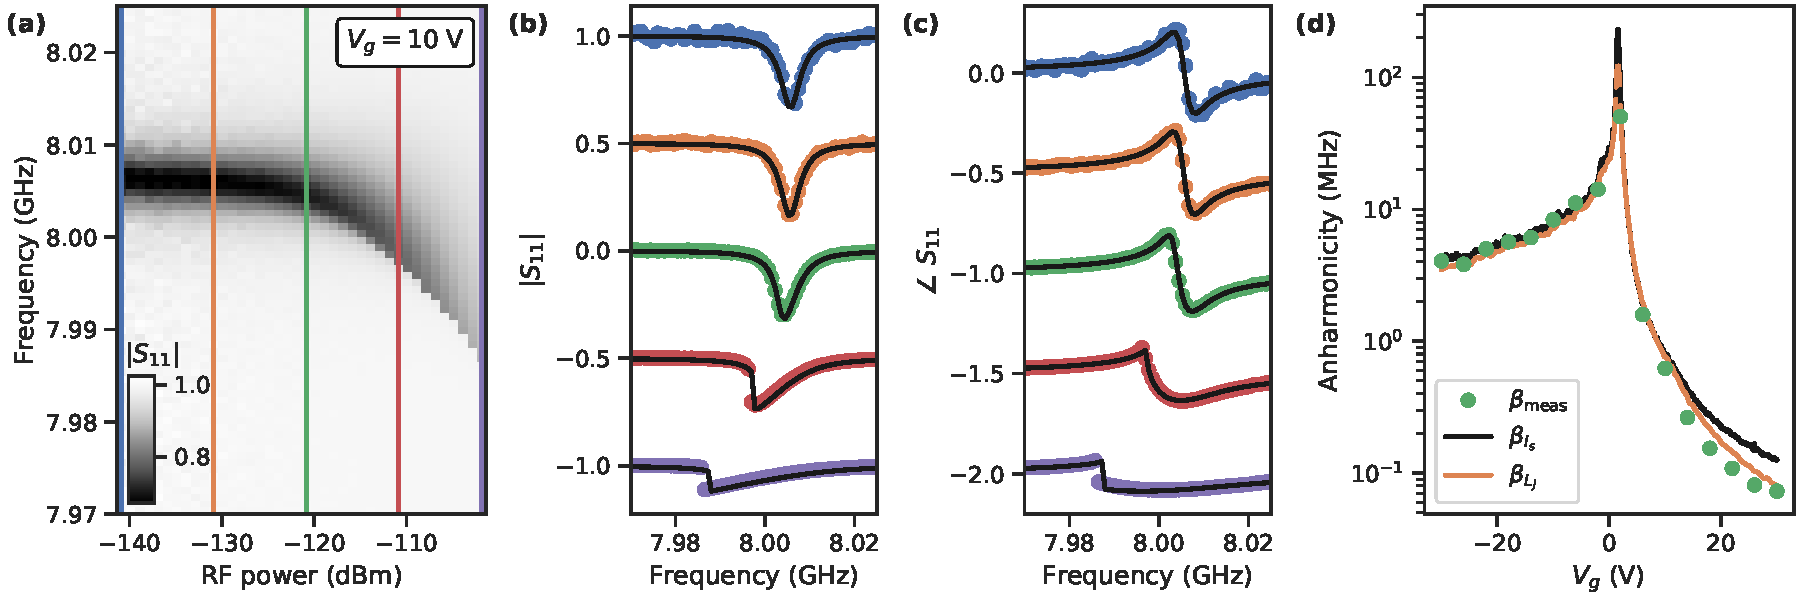
\includegraphics[width=\linewidth]{chapter-gJJ-CPR/figs/Figure4}
	\caption{
		\textbf{Power dependence of a nonlinear microwave device with diffusive gJJ.}
		%
		\textbf{(a)} Absolute value of the reflection coefficient $S_{11}$ versus frequency for increasing drive power.
		%
		Due to the Kerr nonlinearity, the resonator experiences a downshift and bifurcation at elevated drive powers.
		%
		Solid lines indicate linecuts in \textbf{(b)} and \textbf{(c)}.
		%
		\textbf{(b-c)} Absolute value \textbf{(b)} and phase \textbf{(c)} of $S_{11}$ for varying drive power as indicated in \textbf{(a)}.
		%
		Black lines are fits.
		%
		\textbf{(d)} Anharmonicity vs gate voltage.
		%
		Dots: data as extracted from fits as in \textbf{(b-c)}, orange line: model using DC-$I_s$, green: model using RF-$I_c$.
		%
		The overestimation of the anharmonicity of the DC-$I_s$ for high gate voltages hints at a non-sinusoidal CPR.
	}
	\label{fig:figure4}
\end{figure}

\section{Reconstructing the current phase relation}

The current phase relation (CPR) for a ballistic point contact is given by
%
\begin{align}
I_J(\delta,\tau,T) = \frac{\pi\Delta}{2 e R_n} \frac{\sin\delta}{\sqrt{1 - \tau \sin^2\delta / 2}} \tanh\left(\frac{\Delta}{k_B T} \sqrt{1 - \tau \sin^2\delta / 2}\right),
\label{eq:CPR-ball}
\end{align}
%
with the normal state resistance $R_n= R_q/N = h/(Ne^2)\approx \SI{25.812}{\kilo\ohm} / N$~\cite{golubovCurrentphaseRelationJosephson2004a}.
%
Here, $R_q$ denotes the quantum Hall resistance and $N$ the number of conducting channels.
%
With a normal state resistance of or devices ranging between \SIrange{35}{350}{\ohm} (depending on gate voltage), we estimate around 74 to 740 conducting channels.
%
This justifies the use of a single transparency parameter $\tau$ that is the average of all the other channels.
%
Forward skew $S=2\delta_{\rm max}/\pi -1$~\cite{englishObservationNonsinusoidalCurrentphase2016}.
%
%$I_c(\tau,T)=\underaccent{\delta}{\max} \left[I_J(\delta,\tau,T)\right]$
%

\begin{figure}
	\centering
	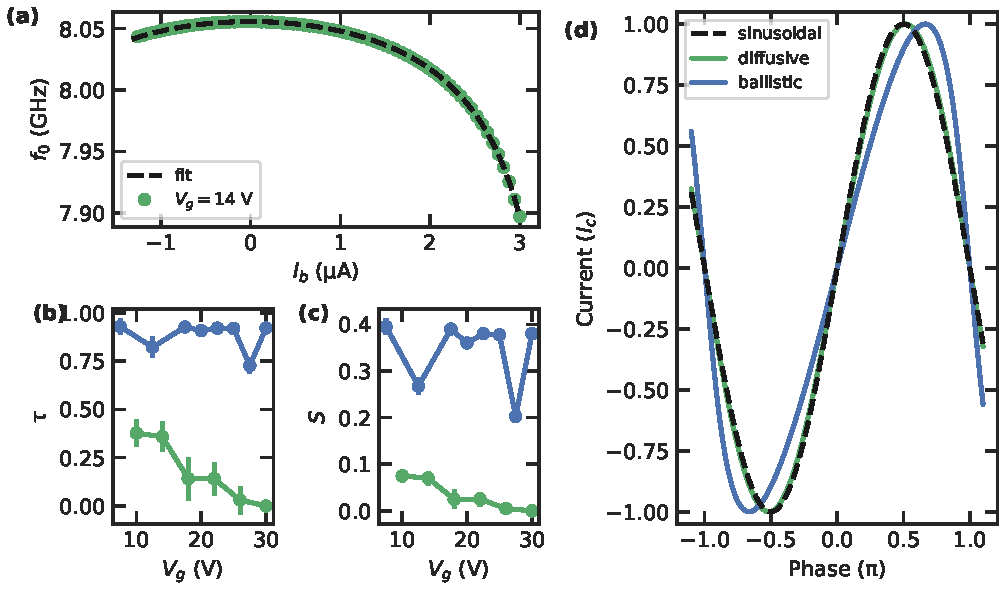
\includegraphics[width=\linewidth]{chapter-gJJ-CPR/figs/Figure5}
	\caption{
		\textbf{Predicted influence of the junction transparency on the bias current dependence.}
		%
		\textbf{(a)} CPR for various $\tau=0$ (solid), $\tau=0.5$ (dashed) and $\tau=1.0$	(dash-dotted).
		%
		\textbf{(b-c)} Josephson inductance \textbf{(b)} and resonance frequency \textbf{(c)} supercurrent for	same transparencies as in \textbf{(a)}.
		%
		Increased junction transmission leads to forward skewing of the CPR, thus a reduced slope and higher Josephson inductance, which in turn reduces the resonance frequency and increases the tuning.
	}
	\label{fig:figure5}
\end{figure}

\begin{figure}
	\centering
	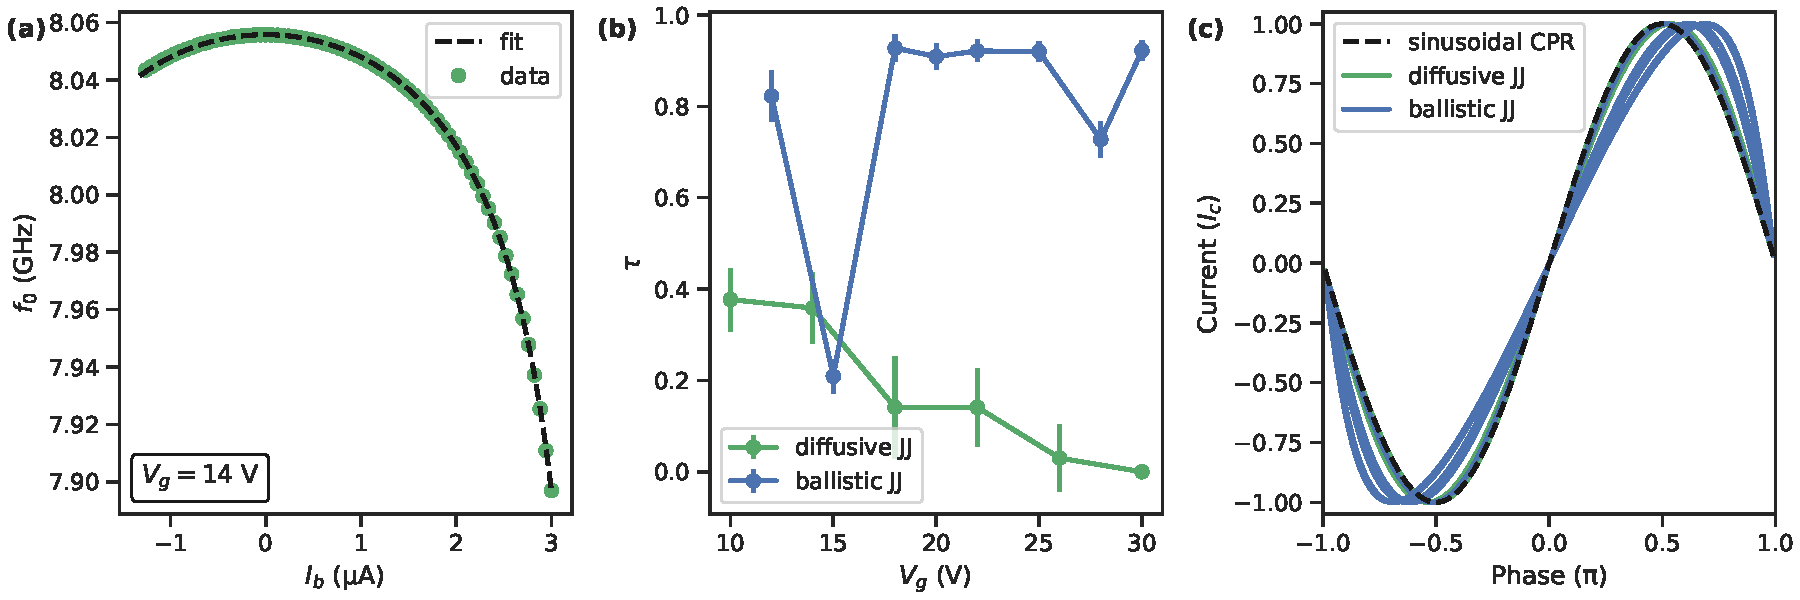
\includegraphics[width=\linewidth]{chapter-gJJ-CPR/figs/Figure6}
	\caption{
		\textbf{Extracting the current phase relation from current-biasing the gJJ microwave circuit.}
		%
		Fitting the bias current dependence \textbf{(a)}, we can extract the junction transparency \textbf{(b)} for the diffusive (green) and ballistic (blue) gJJ device versus gate voltage.
		%
		\textbf{(c)} Reconstructed current-phase relation for the diffusive (green) and ballistic (blue) device.
		%
		The large transparency of the ballistic JJ leads to significant forward skewing, while the relatively low transparency of the diffusive JJ only results in minor skewing.
	}
	\label{fig:figure6}
\end{figure}




\references{dissertation}

